\chapter{Tools implementing software metrics} \label{roz:metrics-tools}

\textit{This chapter describes the tools (part of them are plug-ins for Eclipse IDE) that implements software metrics. Part of them are command-line applications. There are presented not only professional tools provided by software companies, but also created by academic teams and individual developers. The final conclusions and indication of the best tools are in the summary of the chapter. The tools are presented in alphabetical order.} 
%%%%%%%%%%%%%%%%%%%%%%%%%%%%%%%%%%%%%%%%%%%%%%%%%%

\section{C and C++ Code Counter (CCCC)}
CCCC is a command line tool developed by Tim Littlefair. It is freeware and open source interface designed for Linux and Windows platform. Firstly, CCCC were implemented to process C-family language files (C++ and ANSI C), however last versions are able to process Java source files as well. The installation and running process on the command line is rather easy. CCCC checks the extension of name of file, and if the extension is known and indicates a supported language, the appropriate parser runs file analysis. Final output of the analysis is generated in HTML and XML files. Despite the fact, that HTML summary is not eye-catching, it is a readable and clear summary of analysis made by CCCC tool (Figures~\ref{fig:cccc1} and \ref{fig:cccc2}). While the XML version is rather difficult to read, analyse and understand (Listing~\ref{ccccXml}). 

\begin{figure}[h!]
	\centering
	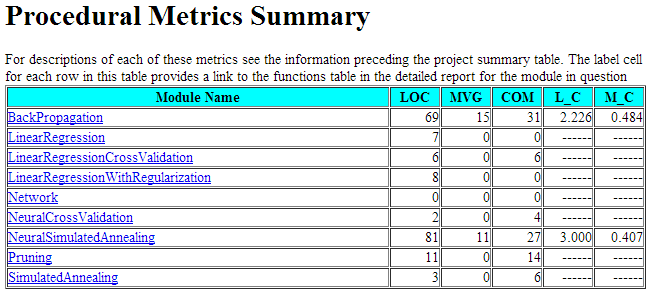
\includegraphics[scale=0.6]{img/cccc1.png} 
	\caption{Procedural metrics summary generated by CCCC metric tool (\ac{NOM}, \ac{COM}, \ac{LC}, \ac{MC})}		
	\label{fig:cccc1}
\end{figure}

\begin{figure}[h!]
	\centering
	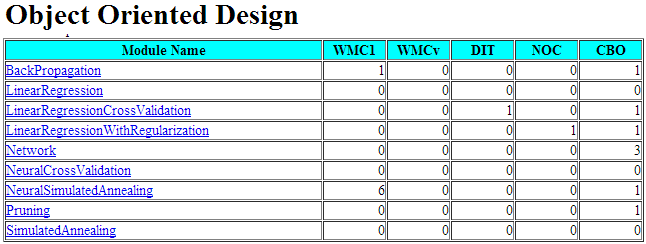
\includegraphics[scale=0.6]{img/cccc2.png} 
	\caption{Object Oriented Design summary generated by CCCC metric tool.}		
	\label{fig:cccc2}
\end{figure}

CCCC produces various measures such as size metrics, complexity metrics, object oriented metrics defined by Chidamber and Kemerer (\cite{indie}, \cite{vaxjo} and \cite{cccc1}).

CCCC could be downloaded from \textit{sourceforge.net} servers\footnote{CCCC download - \url{http://sourceforge.net/projects/cccc/}} and detailed user guide is available on Tim Littlefair official page\footnote{CCCC user guide - \url{http://www.stderr.org/doc/cccc/CCCC\%20User\%20Guide.html}}.

\begin{lstlisting}[caption=XML representation of results generated by CCCC metric tool, label=ccccXml]
<?xml version="1.0" encoding="utf-8"?>
<!--Detailed report on module Network-->
<CCCC_Project>
<module_summary>
<lines_of_code value="0" level="0" />
<lines_of_code_per_member_function value="******" level="0" />
<McCabes_cyclomatic_complexity value="0" level="0" />
<McCabes_cyclomatic_complexity_per_member_function value="******" level="0" />
<lines_of_code value="0" level="0" />
<lines_of_code_per_member_function value="********" level="0" />
<lines_of_code_per_line_of_comment value="------" level="0" />
<McCabes_cyclomatic_complexity_per_line_of_comment value="------" level="0" />
<weighted_methods_per_class_unity value="0" level="0" />
<weighted_methods_per_class_visibility value="0" level="0" />
<depth_of_inheritance_tree value="0" level="0" />
<number_of_children value="0" level="0" />
<coupling_between_objects value="3" level="0" />
...
</CCCC_Project>
\end{lstlisting}

%%%%%%%%%%%%%%%%%%%%%%%%%%%%%%%%%%%%%%%%%%%%%%%%%%%%%%%%%%%
\section{CKJM - Chidamber and Kemerer Metrics}
\textit{CKJM} is an open source command-line tool which calculates object-oriented metrics proposed by Chidamber and Kemerer. This tool processes the byte-code of compiled Java files. 

To run \textit{CKJM} the following line need to be executed\footnote{\textit{CKJM} tool could be download from: \url{http://www.spinellis.gr/sw/ckjm/doc/indexw.html}}:

\begin{verbatim} 
java -jar [localization of ckjm.jar] [localization of *.class files] 
\end{verbatim} 

The command's output will be a list of class names (prefixed by the package they are defined in), followed by the corresponding metrics for that class: \ac{WMC}, \ac{DIT}, \ac{NOC}, \ac{CBO}, \ac{RFC}, \ac{LCOM}, \ac{Ce}, and NPM - number of public methods for a class (last two are not \ac{CK metrics}). The exemplary output is presented below:

\begin{verbatim} 
Algorithms.NeuralSimulatedAnnealing 6 1 0 3 28 0 0 3 2 0,7667 328 0,8333 
0 0,0000 0,3333 0 0 52,6667
 ~ private void changeWeights(): 4
 ~ private double[] changeWeightsArray(double[] weights): 2
 ~ private void feedforward(): 2
 ~ public void annealNetwork(): 4
 ~ public void <init>(NeuronNetworkLibrary.Network network, long cycles, 
 double startingTemp, double stopTemp): 1
 ~ private void revertWeights(): 4
\end{verbatim} 

The form of results presentation is definitely not intelligible and comparing to other tools is rather out-of-date.  


%%%%%%%%%%%%%%%%%%%%%%%%%%%%%%%%%%%%%%%%%%%%%%%%%%
\section{Cobertura}
Cobertura\footnote{Cobertura official page - \url{http://cobertura.github.io/cobertura/}} is a freeware tool that checks code coverage metrics, but it also implements Cyclomatic Complexity.  It uses compiled Java class files and generates output report in XML or HMTL format. Reports shows percentage test coverage on different levels like packages, classes and methods (Figure~\ref{fig:coverage1}). 

\begin{figure}[h!]
	\centering
	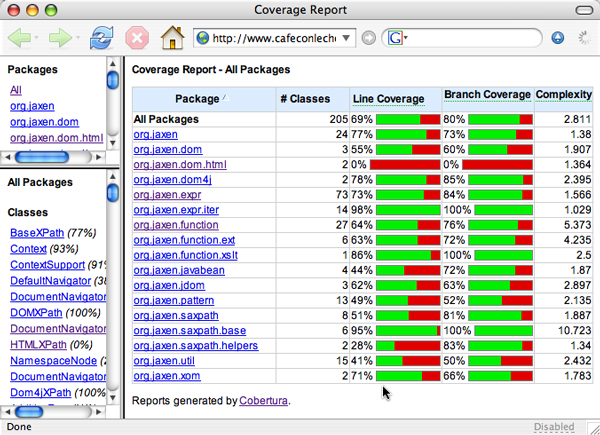
\includegraphics[scale=0.5]{img/coverage.jpg} 
	\caption{HTML report generated by Cobertura (image source: \url{http://tnijurl.com/58c65644bde2/}).}		
	\label{fig:coverage1}
\end{figure}

Cobertura is run with use of command line or Ant task. It is distributed also as a plugin for Eclipse IDE and is named eCobertura (Figure~\ref{fig:coverage2}). 

\begin{figure}[h!]
	\centering
	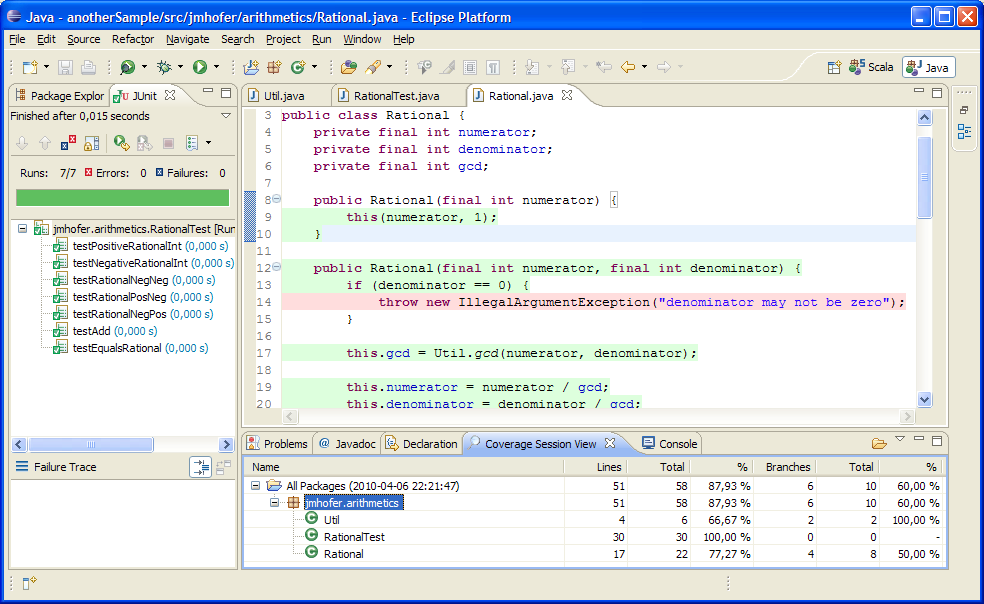
\includegraphics[scale=0.4]{img/screenshot_ecobertura_01.png}  
	\caption{eCobertura as a plug-in for Eclipse IDE (image source: \url{http://ecobertura.johoop.de/}).}		
	\label{fig:coverage2}
\end{figure}


%%%%%%%%%%%%%%%%%%%%%%%%%%%%%%%%%%%%%%%%%%%%%%%%%%%%%%%%%%%
\section{Eclipse Metrics Plug-in 1.3.6}
Eclipse Metrics Plug-in is an open source metrics calculator plug-in for the Eclipse IDE. It detects
cycles in package, dependencies types and measures various metrics like size metrics (\ac{LoC}, number of classes, number of children, number of interfaces), Martin's metrics and \ac{CK metrics}. 

The plug-in is available to download from \textit{sourceforge.net} servers\footnote{Eclipse Metrics Plug-in 1.3.6 official page - \url{http://metrics.sourceforge.net/}.}. In Eclipse, the result of measurement are presented in \textit{Metrics View} where red colour shows which metrics values exceed assumed values and blue one shows which values are accepted (Figure~\ref{fig:eclipsemetrics}). The whole interface is configurable and is handy tool for developers during implementation. 

The results of metrics could be exported to XML file. The scope of the report (project, package, etc.) is selected from context menu.

\begin{figure}[h!]
	\centering
	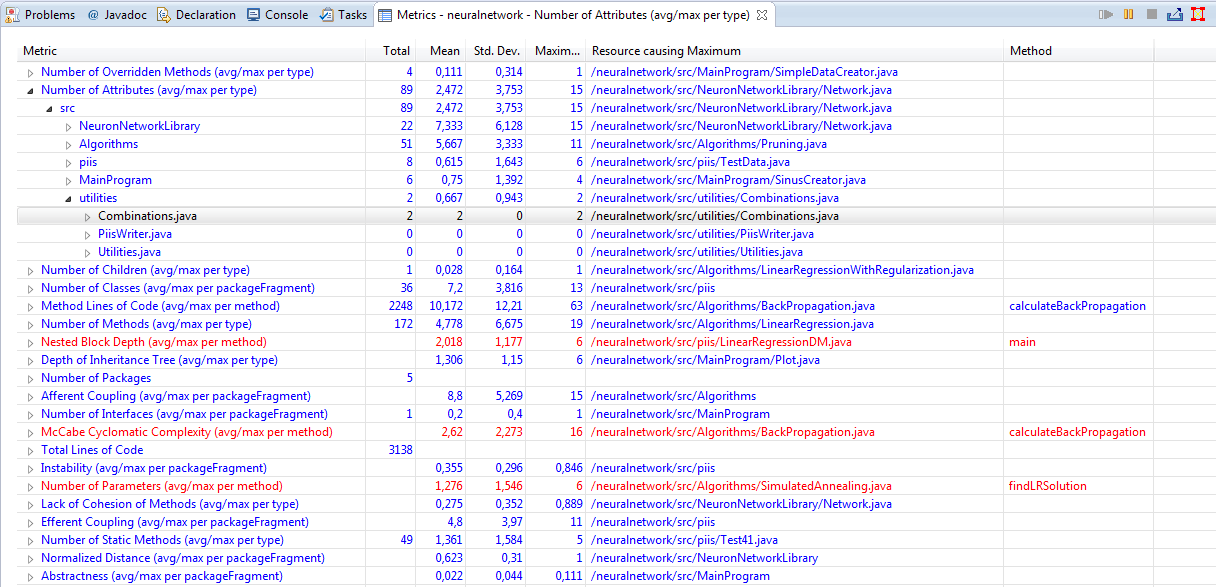
\includegraphics[scale=0.45]{img/eclipse-plugin.png} 
	\caption{Eclipse Metrics Plug-in}		
	\label{fig:eclipsemetrics}
\end{figure}


%%%%%%%%%%%%%%%%%%%%%%%%%%%%%%%%%%%%%%%%%%%%%%%%%%%%
\section{JHawk}
JHawk is shareware metric tool for Java language. It is distributed as stand-alone GUI application or a command line application or as an Eclipse plug-in. The results of measurement is provided in commonly used formats: CSV, XML and HTML. Demo version of JHawk could be downloaded from official website\footnote{JHawk official page - \url{http://www.virtualmachinery.com/jhawkprod.htm}}.

JHawk is advanced measurement tool. The GUI or plugin version provides a dashboard tab which gives overview of the metrics at System, Package and Class level, so the interface is really intuitive and user-friendly. The data are presented in readable and intelligible way. What is more, this tool enables also to create own metrics.

JHawk implements size metrics: Lines of Code, Lines of Comments, Lines of Statements and Expressions; complexity metric created by Halstead (Halstead metrics) and object-oriented metrics created by Chidamber and Kemerer. 

\begin{figure}[h!]
	\centering
	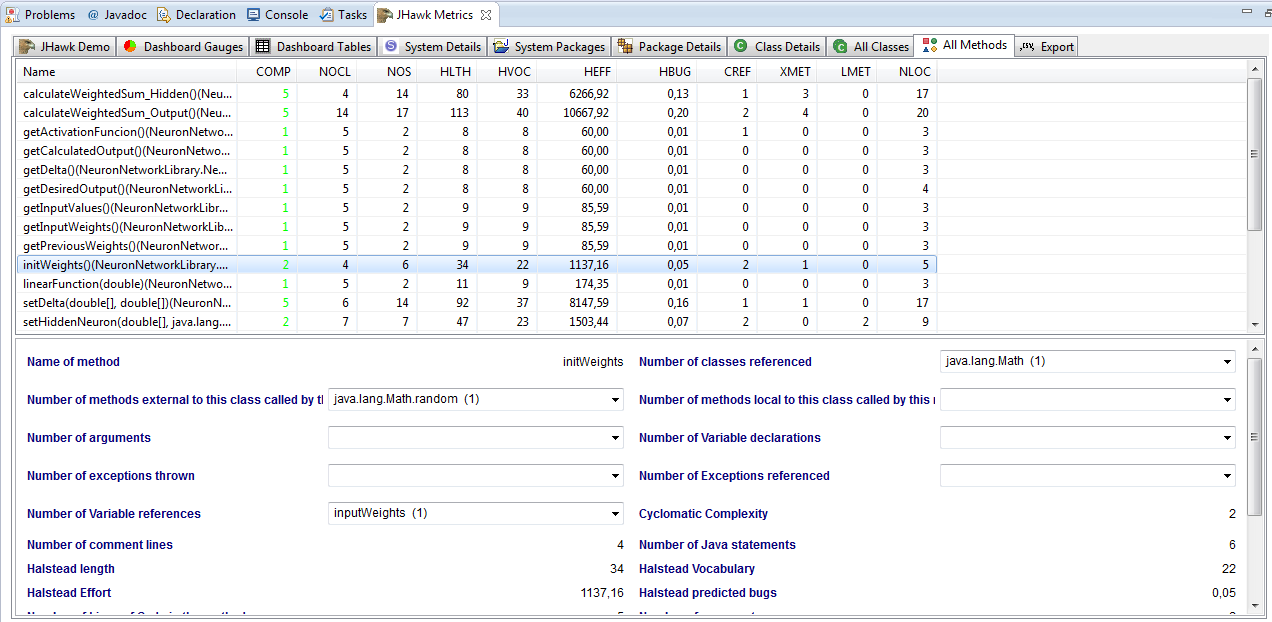
\includegraphics[scale=0.45]{img/jhawk1.png} 
	\caption{JHawk: All Methods View}		
	\label{fig:jhawk1}
\end{figure}

\begin{figure}[h!]
	\centering
	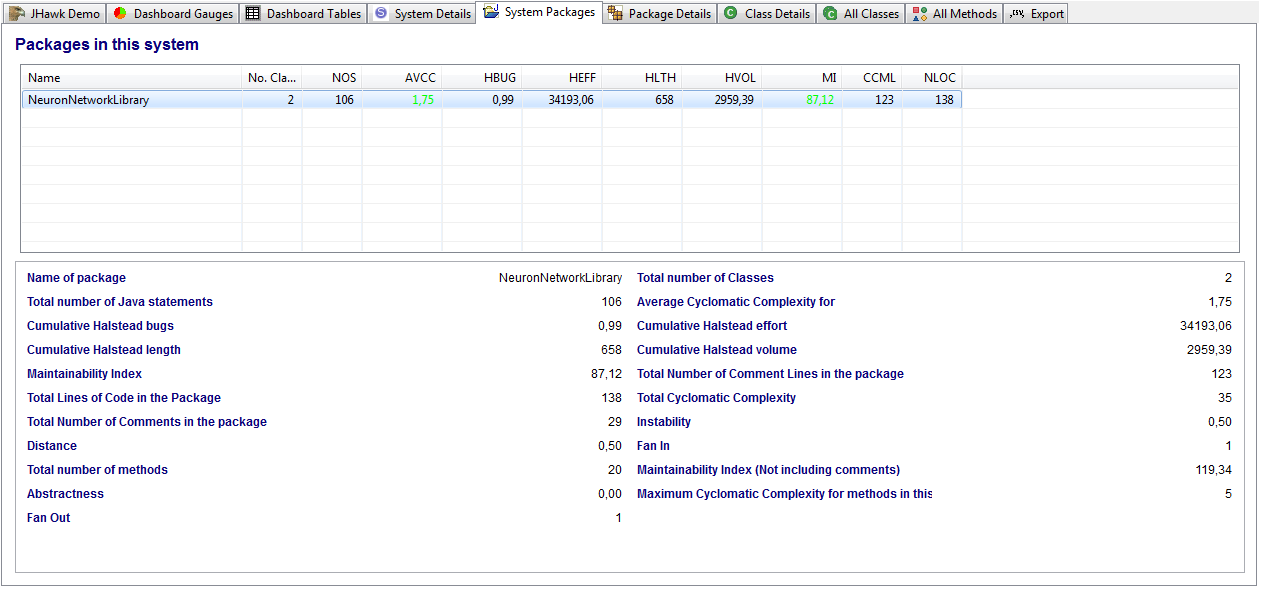
\includegraphics[scale=0.45]{img/jhawk2.png}  
	\caption{JHawk: System Packages View}		
	\label{fig:jhawk2}
\end{figure}

%%%%%%%%%%%%%%%%%%%%%%%%%%%%%%%%%%%%%%%%%%%%%%%
\section{RefactorIT}
RefactorIT provides not only source-code metrics, but also supports automated refactoring process, audits and corrective actions. It is installed as a stand-alone application or as a plug-in to Eclipse or NetBeans. It was commercial tool developed by Aqris company. Since 2008, the RefactorIT is an abandoned project and is freely accessed.  

The plug-in is still available to download on \textit{sourceforge.net} servers\footnote{RefactorIT official page - \url{http://refactorit.sourceforge.net/}.}. The detailed user guide has been prepared by the student of Pennsylvania University\footnote{RefactorIT user guide - \url{http://tnijurl.com/0472430909e9/}.}.  

RefactorIT implements large set of metrics:
\begin{itemize}
\item size metrics: \ac{LoC}, \ac{CLOC}, \ac{DC}, \ac{EXEC}, \ac{NOT}, \ac{NOTa}, \ac{NOTc}, \ac{NP}, \ac{NOF}, \ac{NOA} (description of these metrics in section~\ref{sec:other-metrics}).
\item complexity metric:~\ac{CC}
\item Martin's metrics
\item \ac{CK metrics} without \ac{LCOM} and \ac{CBO}.
\end{itemize}
 
RefactorIT generates a report in text, HTML and XML format with values from all selected metrics analyse for all types of level. It gives the possibility of further analysis of metrics based on all the values collected from the entire project or selected package, component or module. 
 
In Eclipse IDE, the values of metrics that  exceeded admissible values are marked on red (Figure~\ref{fig:refactor2}). The exceeded values are also changeable and could be set before starting process of metrics measurement (Figure~\ref{fig:refactor1}). 
 
\begin{figure}[h!]
 	\centering
 	 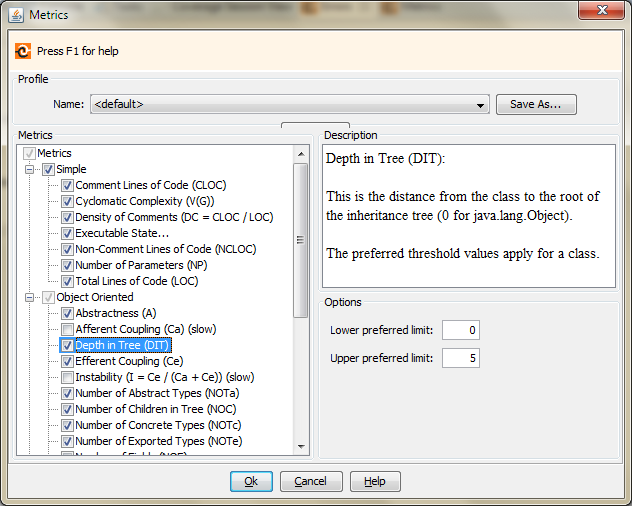
\includegraphics[scale=0.6]{img/refactorit1.png} 
 	\caption{RefactorIT: choice of metrics used to prepare a final measurement report, there is also a short description of each metrics.}		
 	\label{fig:refactor1}
 \end{figure} 

\begin{figure}[h!]
	\centering
	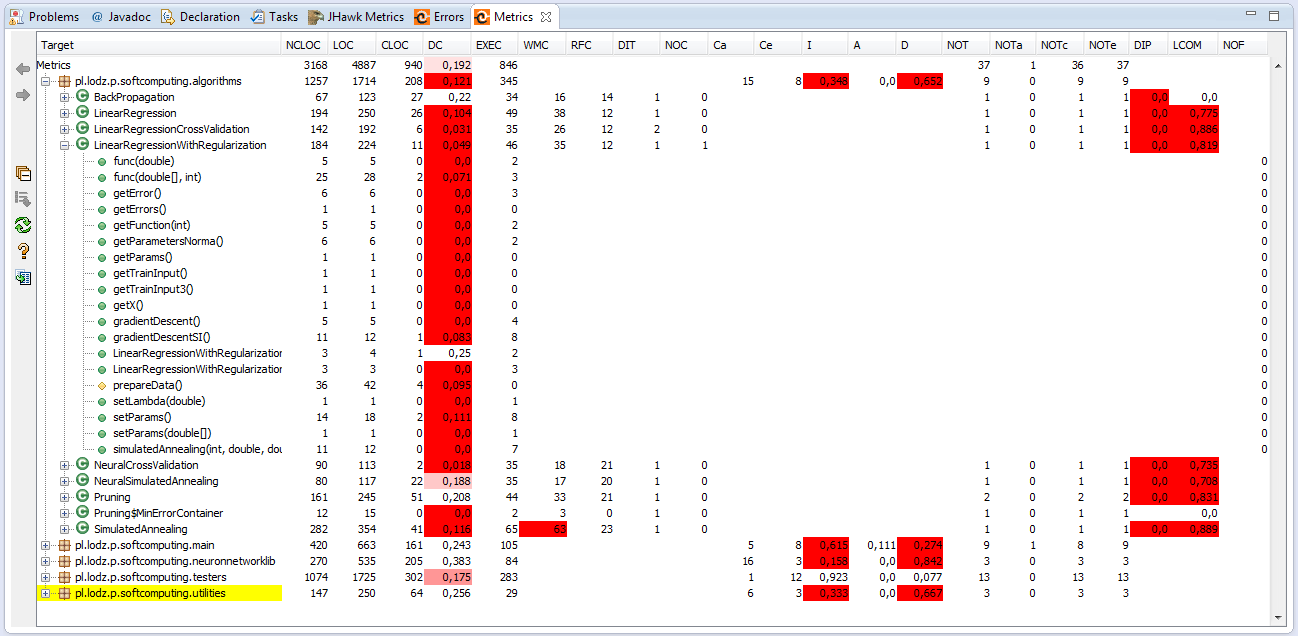
\includegraphics[scale=0.45]{img/refactorit2.png}  
	\caption{RefactorIT: the results of metrics measurement in Eclipse IDE.}		
	\label{fig:refactor2}
\end{figure}

%%%%%%%%%%%%%%%%%%%%%%%%%%%%%%%%%%%%%%%%%%%%%%%%%
\section{SonarQube (Sonar)}
SonarQube (previously known as \textit{``Sonar''}) is open-source platform used to maintain a quality of software. Originally, it was designed to analyse software written in Java, but set of additional plug-ins extends possibility to support: Android, C, C++, Cobol, C Sharp, Flex, JavaScript, PHP, PL/SQL and Visual Basic. Nowadays, it is the fastest developing platform that supports code metrics. It is used by many software companies and programmer teams. It is fully integrated with Maven, Ant, continuous integration tools (Atlassian Bamboo, Jenkins), IDEs (Eclipse) and bug tracking systems (JIRA).    

The installation files are ready to download from official page of SonarQube\footnote{SonarQube official page - \url{http://www.sonarqube.org}.}. It is also required to install server environment (Tomcat) and database. 

The set of metrics supported in SonarQube is also very rich:

\begin{itemize}
\item size metrics:  \ac{LoC}, \ac{COM}, \ac{DC}, \ac{NOM}, \ac{EXEC}, number of classes,  number of methods, number of getters and setters methods and code coverage (description of some of these metrics in sections~\ref{sec:other-metrics} and~\ref{sec:codecoverage}).
\item complexity metric:~\ac{CC}
\item \ac{CK metrics}
\item Martin's metrics: \ac{Ca} and \ac{Ce} metric.
\end{itemize}

The main advantages of SonarQube are efficient way of navigating and elaborated balance in high-level view of dashboard supporting in faults detection (Figure~\ref{fig:sonar1}). What is more, it is a web-based application, so the overall rules, alerts, exclusions, settings are configurable in web browser. It not only allows to combine metrics altogether, but also to mix them with chronological measures (Figure~\ref{fig:sonar2}).

\begin{figure}[h!]
	\centering
	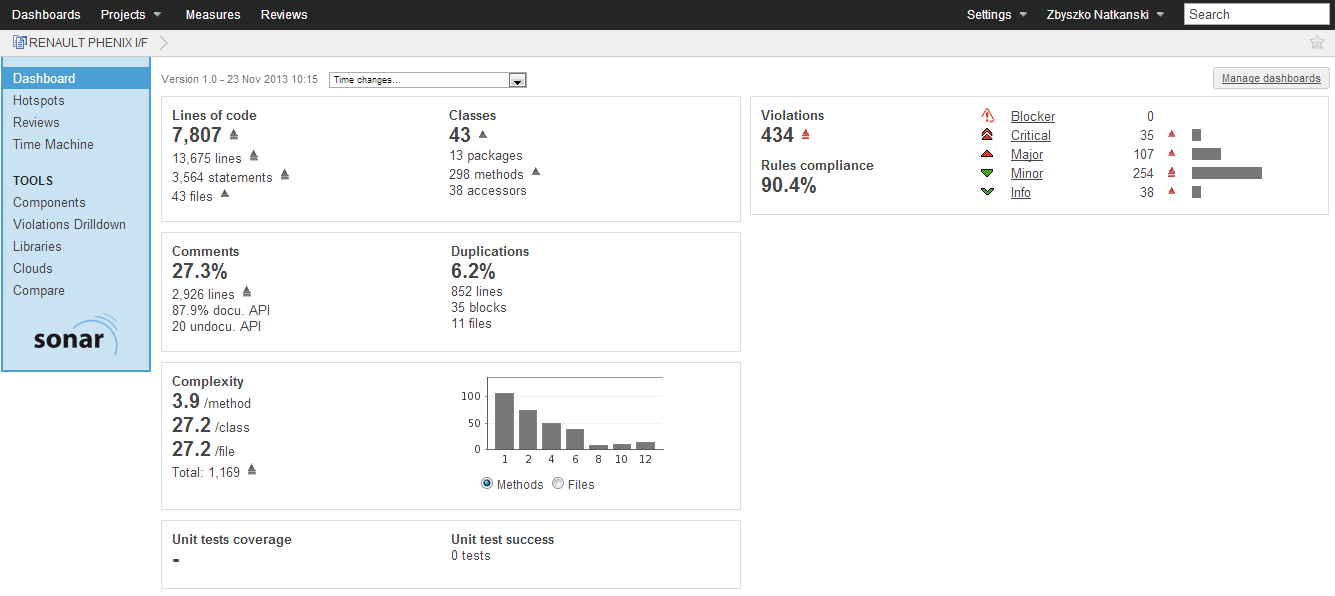
\includegraphics[scale=0.45]{img/sonar2.png} 
	\caption{SonarQube dashboard.}		
	\label{fig:sonar1}
\end{figure}


\begin{figure}[h!]
	\centering
	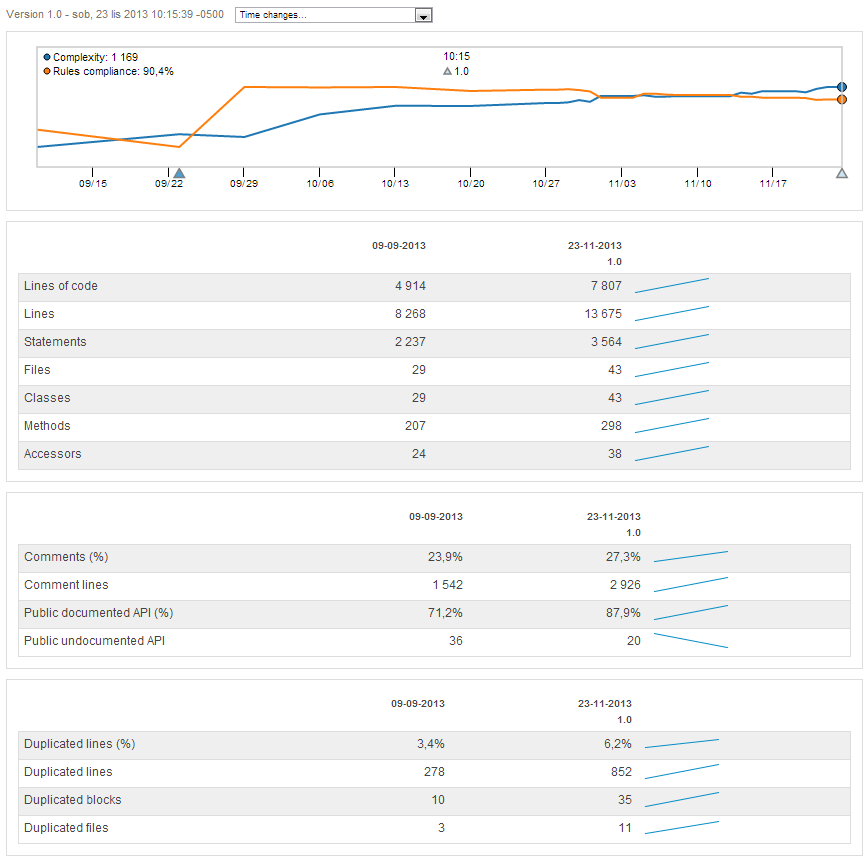
\includegraphics[scale=0.45]{img/sonar4.png} 
	\caption{SonarQube chronological metrics measurement.}		
	\label{fig:sonar2}
\end{figure}



%%%%%%%%%%%%%%%%%%%%%%%%%%%%%%%%%%%%%%%%%%%%%%%%%%
\section{SourceMonitor}
SourceMonitor (SM) is measurement metric tool developed by Campwood software. It has graphical user interface and is a freeware closed-source software which runs only on Windows. There are five different views available to display the results: checkpoint, charts, project, details and method view (Figure~\ref{fig:sourcemonitor}). There are multiple supported languages like Visual Basic, HTML, C, C++, Java, and .NET platform languages family. The results of measurements are exported to XML or CSV format files. The implemented metrics are \ac{LoC}, the ratio of methods per class, number of classes and interfaces, Cyclomatic Complexity, the percentage ratio of statements and \ac{LoC} and percentage ratio of commented lines (\cite{indie}).

SourceMonitor is available to download on official website\footnote{SourceMonitor download - \url{http://www.campwoodsw.com/sourcemonitor.html}}.

\begin{figure}[h!]
	\centering
	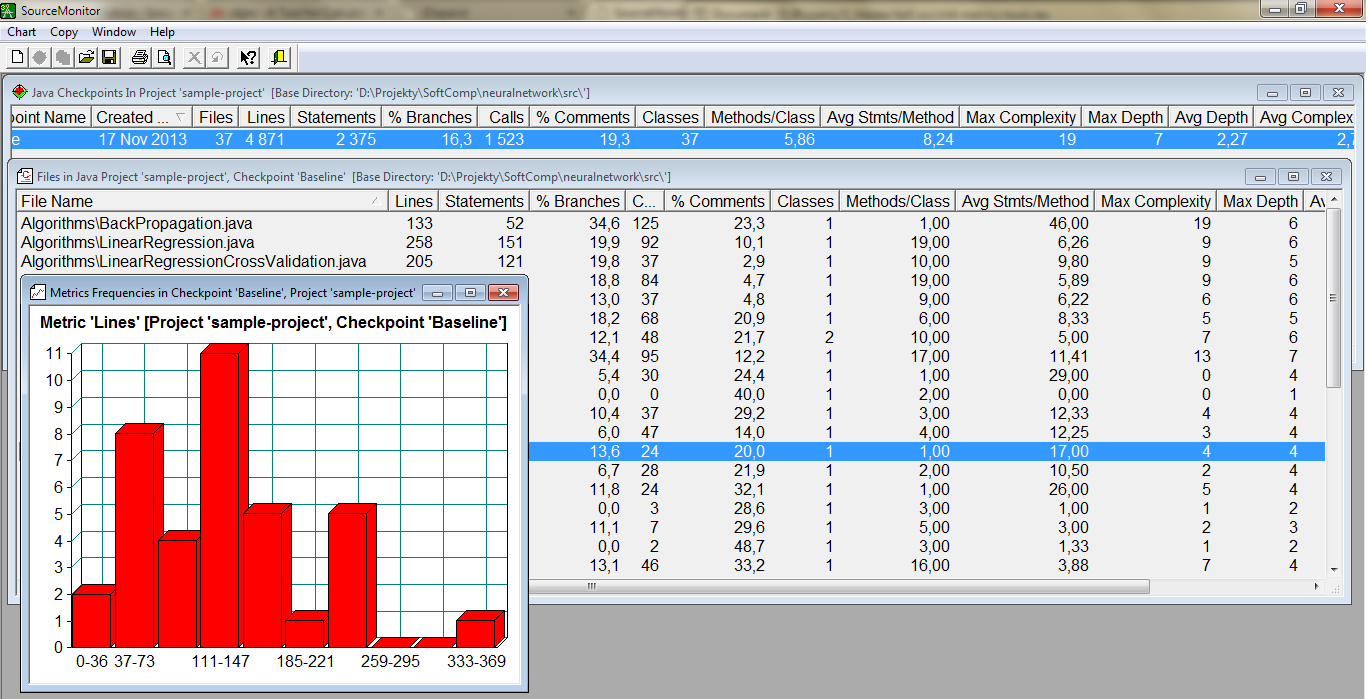
\includegraphics[scale=0.4]{img/sourcemonitor.png} 
	\caption{SourceMonitor metric tool.}		
	\label{fig:sourcemonitor}
\end{figure}

%%%%%%%%%%%%%%%%%%%%%%%%%%%%%%%%%%%%%%%%%%%%%%%%%%%%%%%%%%%
\section{STAN - Structure Analysis for Java} 
STAN - Structure Analysis for Java is a tool used to structure analysis for Java language. It visualizes project design and reports its flaws. It supports in code understanding and measure the quality. STAN offers also set of selected metrics that underline essential aspects of code quality. All faults are clearly visualized what is a key feature for non technical target clients. This tool is used by developers to take care of code quality from the beginning. It could be used by project managers as a tool for monitoring and reporting. 

STAN tool could be downloaded from official website\footnote{STAN official page - \url{http://www.stan4j.com/}}. It is distributed under the community license option without installing a license key for projects up to 100 classes. There are two variants of product: either standalone application or Eclipse IDE plug-in.

One of the key feature of STAN is computing several metrics. It maps some kinds of artefacts to numbers. The implemented metrics are:

\begin{itemize}
\item size metrics.
\item McCabe's Cyclomatic Complexity
\item Martin's metrics
\item \ac{CK metrics}
\end{itemize}

Metric violations are prioritized  by weighting its rating with the amount of the artifact's underlying code. The results are showed in the violations view (Figure~\ref{fig:stan}).

Another interesting feature is customizable reports generation. It gives a detailed lists of metric violations in colourful visualized pie chars and underline bad trends in project design\footnote{Sample report is presented here:~\url{http://stan4j.com/sample-report.html}}\cite{stan}.

\begin{figure}[h!]
	\centering
	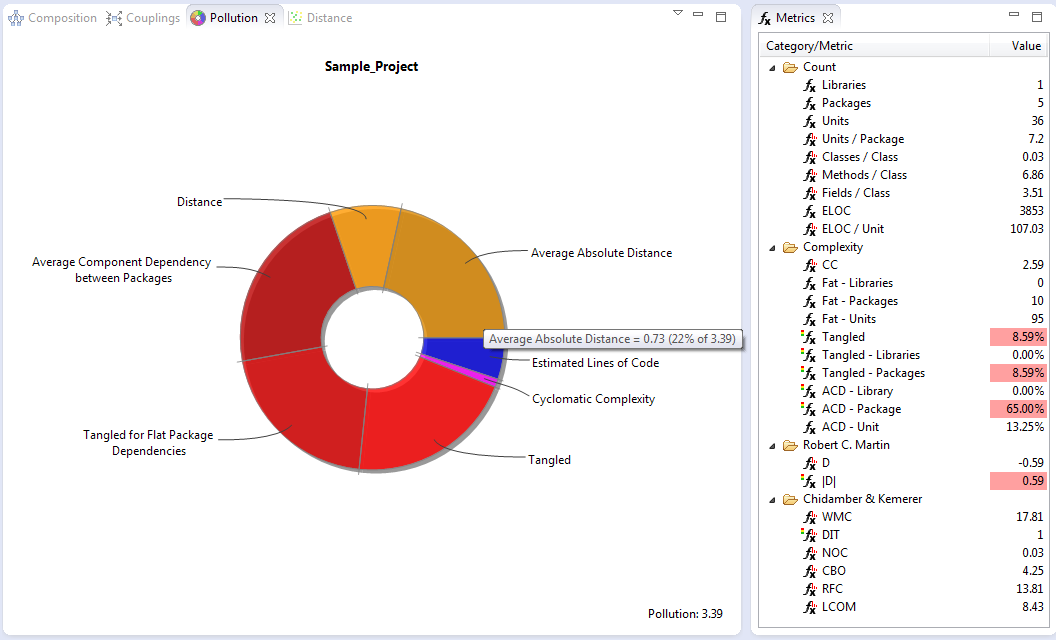
\includegraphics[scale=0.55]{img/stan.png} 
	\caption{STAN - Structure Analysis for Java plug-in for Eclipse IDE.}		
	\label{fig:stan}
\end{figure}
%%%%%%%%%%%%%%%%%%%%%%%%%%%%%%%%%%%%%%%%%%%%%%%%%%

\section{Summary}

%Dodac trzy/dwa z tych dokumentów!!!
%section{JDepend}
%[opis]-delete

%O tych poniżej może tylko wspomnieć¸ ale niekoniecznie.
%tion{Findbugs}
%ion{Checkstyle}
%ction{PDM}
%ction{Simian - Similarity analyser}